\documentclass[10pt,xcolor=pdflatex]{beamer}
\usepackage{newcent}
\usepackage[utf8]{inputenc}
\usepackage[czech]{babel}
\usepackage{hyperref}
\usepackage{fancyvrb}
\usetheme{FIT}

%%%%%%%%%%%%%%%%%%%%%%%%%%%%%%%%%%%%%%%%%%%%%%%%%%%%%%%%%%%%%%%%%%
\title[Bakalářská práce]{Android aplikace pro Git s podporou git-lfs a git-annex}

\author[]{autor práce: Petr Marek\\vedoucí práce: RNDr. Marek Rychlý, Ph.D.}

\author{\texorpdfstring{
    Petr Marek \\
    \footnotesize{vedoucí práce: RNDr. Marek Rychlý, Ph.D.}
}{Petr Marek, vedoucí práce: RNDr. Marek Rychlý, Ph.D.}}

\institute[]{Fakulta informačních technologií VUT v Brně\\
Bo\v{z}et\v{e}chova 1/2. 612 66 Brno - Kr\'alovo Pole\\}

%\date{January 1, 2016}
%\date{\today}
\date{} % bez data

%%%%%%%%%%%%%%%%%%%%%%%%%%%%%%%%%%%%%%%%%%%%%%%%%%%%%%%%%%%%%%%%%%

\begin{document}

\frame[plain]{\titlepage}

\begin{frame}\frametitle{Cíl práce}
    \begin{itemize}
        \item{Git, git-lfs a git-annex}
        \item{Uživatelsky přívětivé rozhraní}
        \item{Minimalizace velikosti repozitářů}
        \item{Rozšiřitelnost}
    \end{itemize}
\end{frame}

\begin{frame}\frametitle{Návrh a implementace}
    \begin{columns}
        \column{0.5\textwidth}
            \begin{itemize}
                \item{Architektura}
                \item{Integrace Gitu}
                \item{Uživatelské rozhraní}
            \end{itemize}
        \column{0.4\textwidth}
            \frame{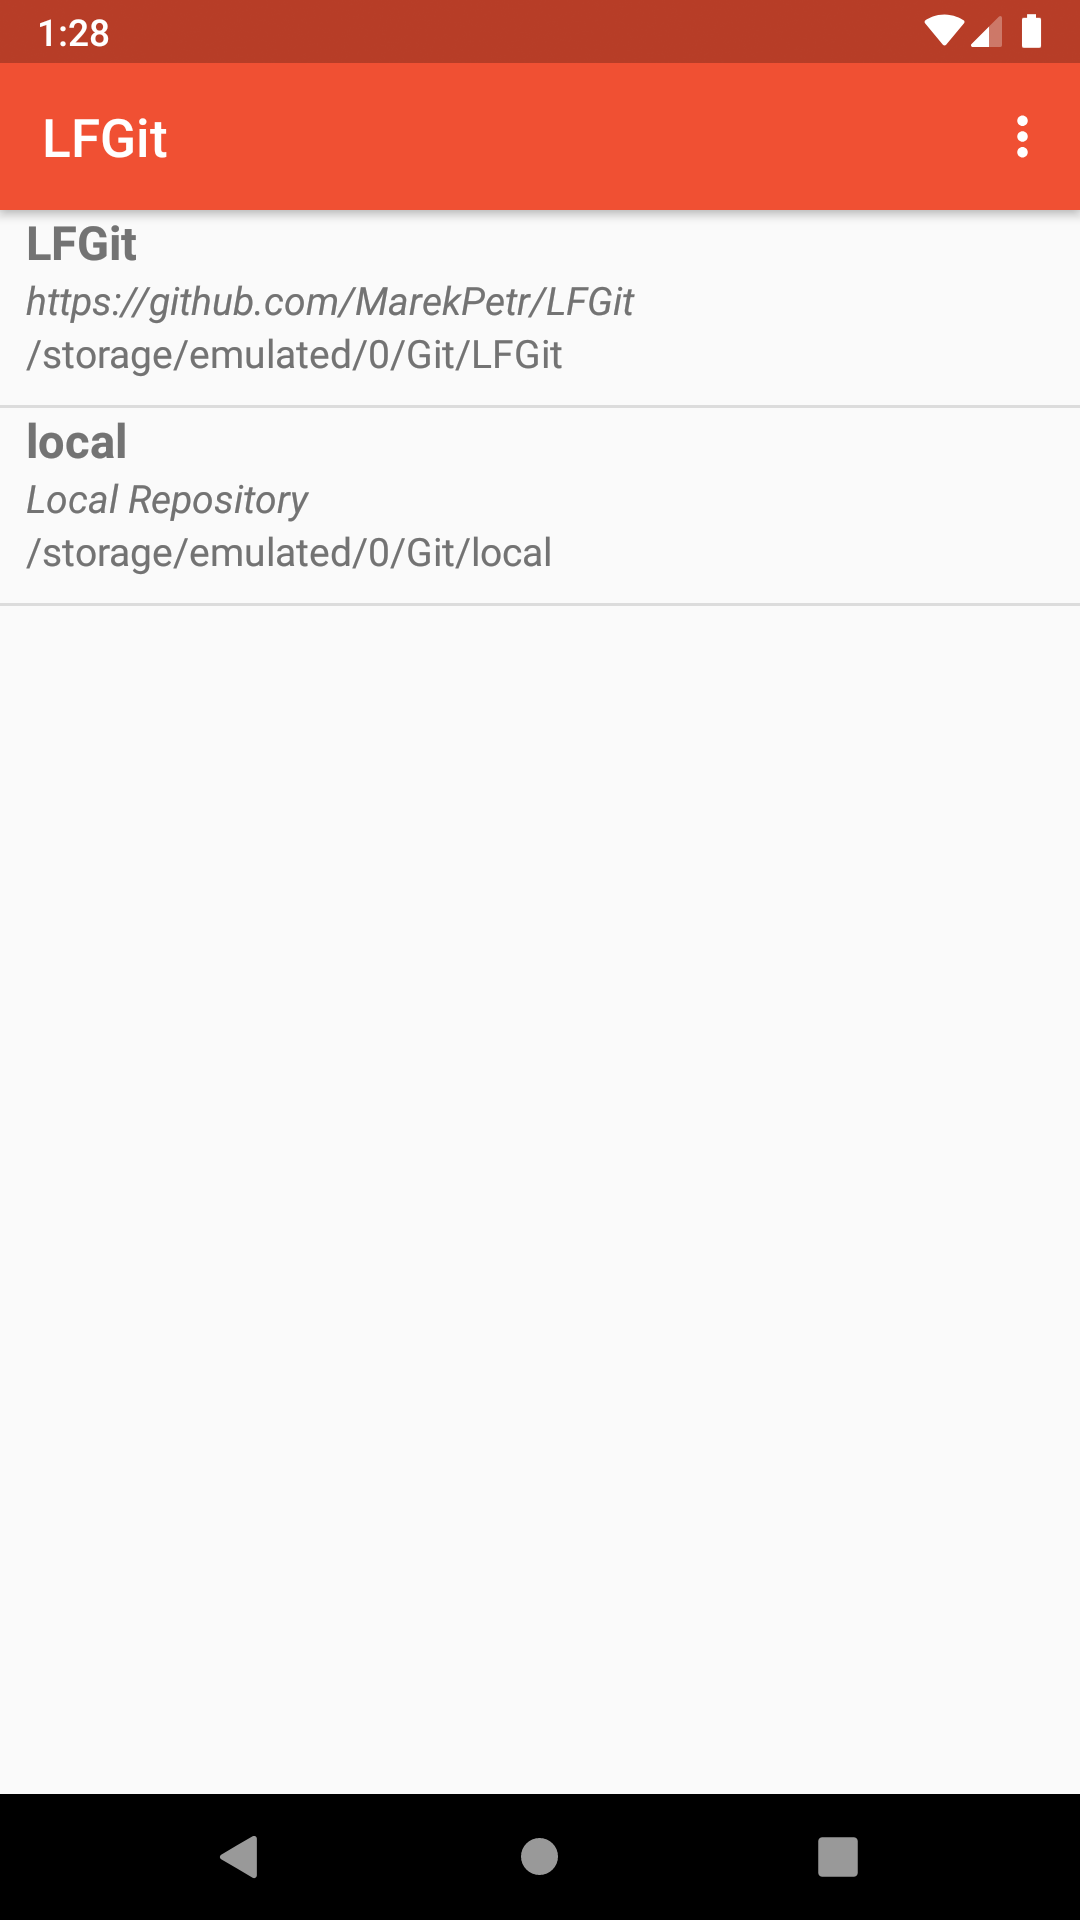
\includegraphics[scale=0.08]{img/repo_list}}
    \end{columns}
\end{frame}

\begin{frame}\frametitle{Výsledná aplikace}
    \begin{columns}
        \column{0.5\textwidth}
            \begin{itemize}
                \item {Funkcionalita}
                \item {Minimalizace velikosti repozitářů}
                \item {Srovnání s konkurencí}
                \item {Možná rozšíření}
            \end{itemize}
        \column{0.4\textwidth}
            \frame{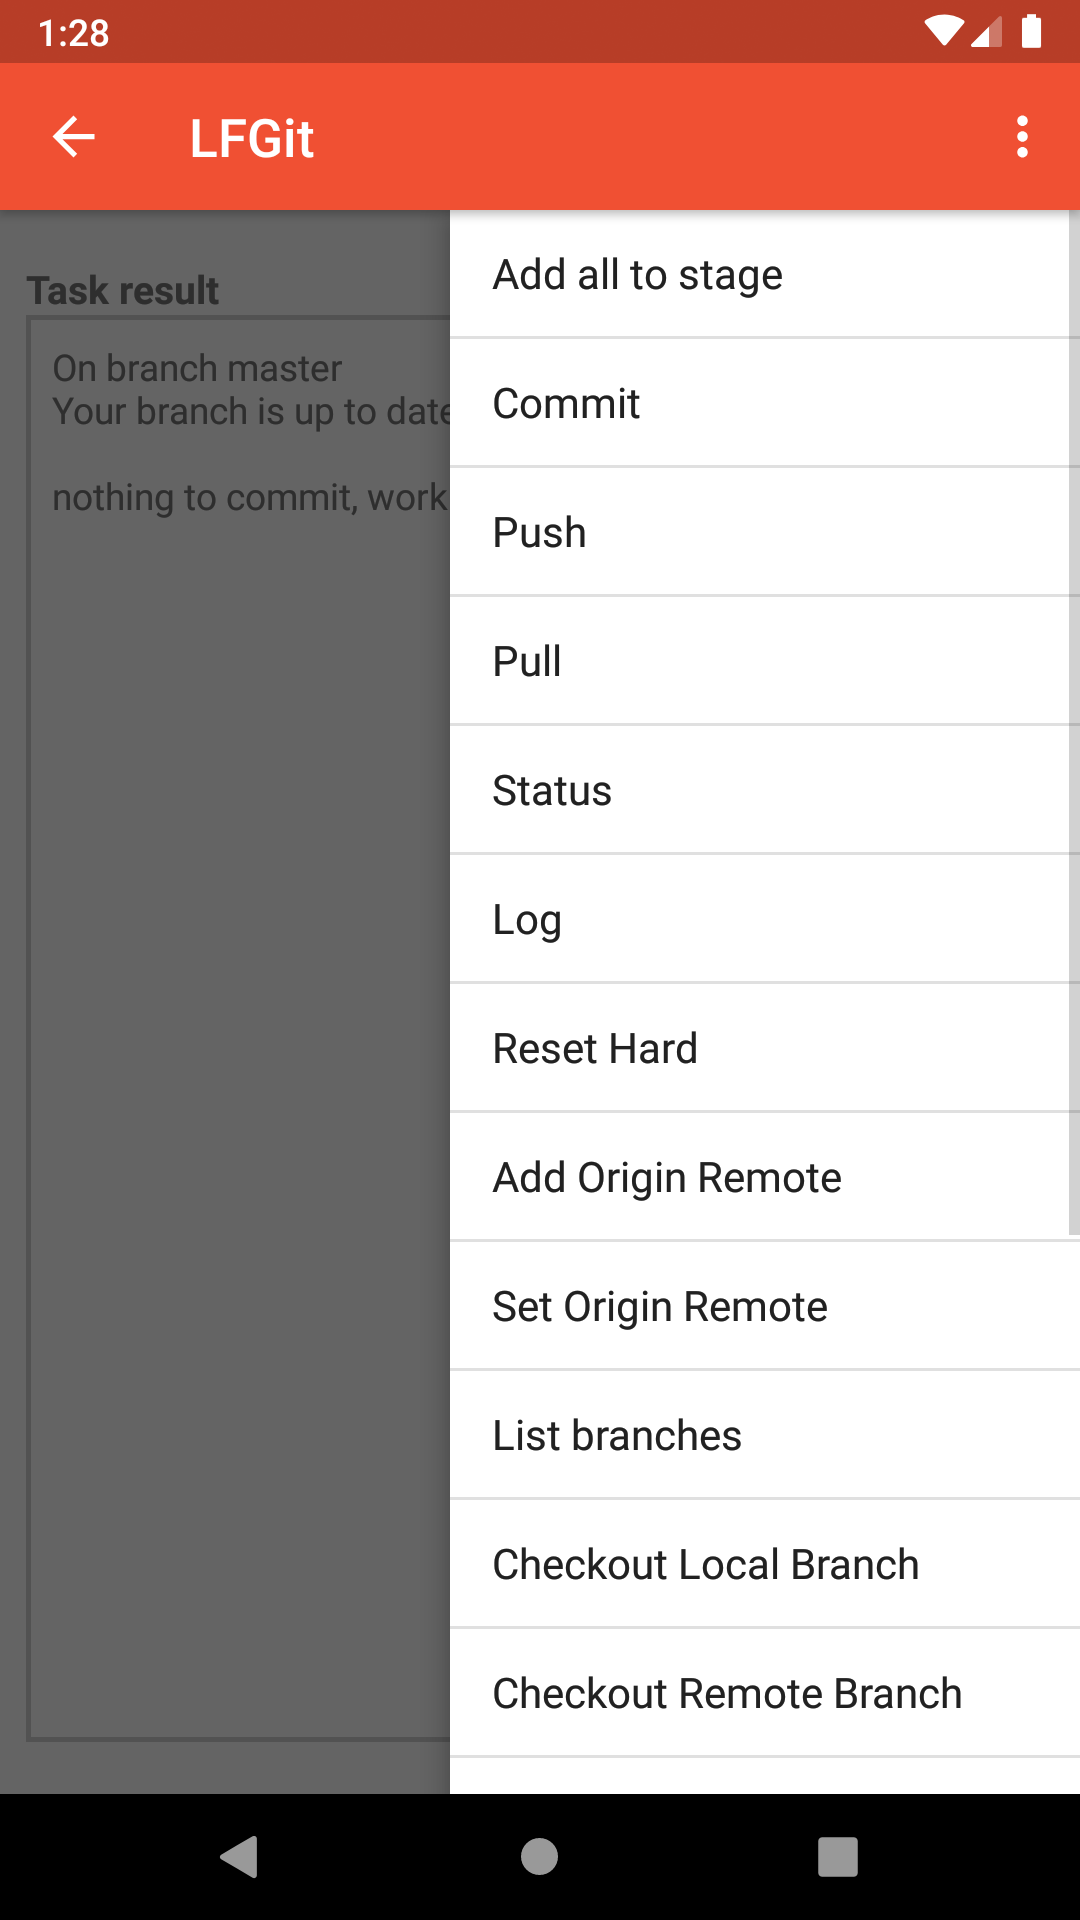
\includegraphics[scale=0.08]{img/tasks}}
    \end{columns}
\end{frame}

\begin{frame}\frametitle{Otázky oponenta a diskuze}
    \begin{itemize}
        \item{Je třeba uchovávat v databázi aplikace jiné údaje, než cesty k repozitářům? Nejsou už ostatní údaje součástí repozitářů?}
        \item{Můžete vysvětlit roli nástrojů docker a termux-packages ve~Vašem řešení?}
        \item{Další otázky...}
    \end{itemize}
    \vspace{0.7cm}
    \begin{figure}[b]
        \frame{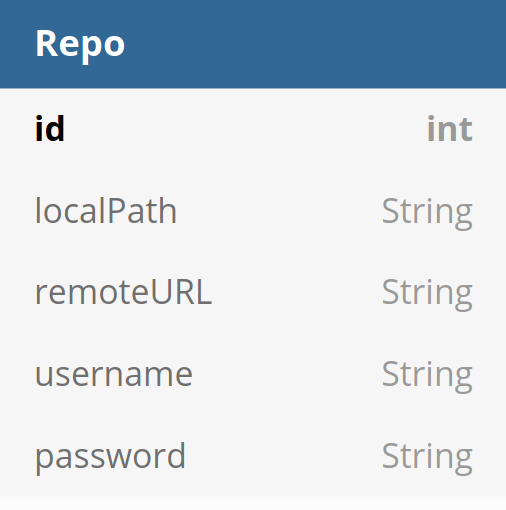
\includegraphics[scale=0.15]{img/repo}}
    \end{figure}
\end{frame}
\end{document}
